\documentclass[11pt, oneside]{article}   	% use "amsart" instead of "article" for AMSLaTeX format
\usepackage{geometry}
\usepackage{amsmath}              		% See geometry.pdf to learn the layout options. There are lots.
\geometry{letterpaper}                   		% ... or a4paper or a5paper or ... 
%\geometry{landscape}                		% Activate for for rotated page geometry
%\usepackage[parfill]{parskip}    		% Activate to begin paragraphs with an empty line rather than an indent
\usepackage{graphicx}				% Use pdf, png, jpg, or eps§ with pdflatex; use eps in DVI mode
								% TeX will automatically convert eps --> pdf in pdflatex		
\usepackage{amssymb}
\usepackage{mcode}

\title{CS 6220 - Final Project: Selection 2}
\author{Ally Warner}
%\date{}							% Activate to display a given date or no date

\begin{document}
\maketitle

\section{Purpose/Statement of Problem}

Consider the following system:

\begin{align*}
-\nabla^2 u(x,y) &= f(x,y) (x,y) \in (0,1) \times (0,1)\\
u(0,y) &= g_1(y); \text{ }y \in [0,1]\\
u(1,y) &= g_2(y); \text{ } y\in [0,1]\\
u(x,0) &= g_3(x); \text{ } x\in [0,1]\\
u(x,1) &= g_4(x); \text{ }x \in [0,1]\\
\end{align*}

Develop a finite element solver to solve the problem above. Assume that piecewise linear $C^0$ global basis functions constructed on triangular tessellations are used. Use a union-jack mesh configuration for all experiments.

\vspace{5mm}

Demonstrate the convergence rate of your method using the following known solution:

\[
u(x,y) = \sin(2\pi x)\sin(2\pi y)
\]

from which the right-hand-side and boundary conditions can be derived. Provide both the rate of convergence when you compute the right-hand-side exactly (to machine precision) and when you approximate the right-hand-side integrals by only sampling the forcing function at the center of the triangles.

\vspace{5mm}

Then solve the above system with:

\begin{align*}
f(x,y) &= 1.0; \text{ } (x,y) \in (0,1) \times (0,1)\\
g_1(y) &= 0.0; \text{ } y \in [0,1]\\
g_2(y) &= 1.0; \text{ } y \in [0,1]\\
g_3(x) &= x; \text{ } x \in [0,1]\\
g_4(x) &= x; \text{ } x \in [0,1]\\
\end{align*}

with spacings of $\frac{1}{5}$, $\frac{1}{10}$, $\frac{1}{20}$, $\frac{1}{40}$ and $\frac{1}{80}$, with the two right-hand-side computations mentioned above.

\section{Description of Mathematics}

The system we are solving is Poisson's equation,
\[
-\nabla^2 u(x,y) = f(x,y) \text{ where } (x,y) \in (0,1) \times (0,1).
\]

Poisson's equation in terms of a Cartesian coordinate system becomes 
\[
\frac{\partial^2 u}{\partial x^2} + \frac{\partial^2 u}{\partial y^2} = g(x,y)
\]

in the two-dimensional domain $\Omega$ which is broken up into discrete elements to form the finite dimensional domain $\Omega_h$. So in the first system,
\[
-f(x,y) = 8 \pi^2 \sin(2 \pi x)(2 \pi y).
\]

We are constructing a mesh using triangular tessellations so we represent our function as such,
\[
u \approx \tilde{u} = \alpha_1 + \alpha_1 x + \alpha_3 y.
\]
We will begin to solve this system one triangle at at time, so we will take out a specific triangle from our discretized domain and apply the above equation to the vertices of the triangle giving the following equations,
\begin{align*}
\tilde{u_1} &= \alpha_1 + \alpha_1 x_1 + \alpha_3 y_1\\
\tilde{u_2} &= \alpha_1 + \alpha_1 x_2 + \alpha_3 y_3\\
\tilde{u_3} &= \alpha_1 + \alpha_1 x_3 + \alpha_3 y_3\\
\end{align*}

With this system, we can solve for the coefficients $\alpha_1$, $\alpha_2$,  and $\alpha_3$ with the following equations,
\begin{align*}
\alpha_1 &= (a_1 \tilde{u_1} + a_2 \tilde{u_2} + a_3 \tilde{u_3})/2A\\
\alpha_2 &= (b_1 \tilde{u_1} + b_2 \tilde{u_2} + b_3 \tilde{u_3})/2A\\
\alpha_3 &= (c_1 \tilde{u_1} + c_2 \tilde{u_2} + c_3 \tilde{u_3})/2A\\
\end{align*}
where 
\begin{align*}
a_1 &= x_2 y_3 - x_3 y_2\\
b_1 &= y_2 - y_3\\
c_1 &= x_3 - x_2\\
2A &= a_i +b_i x_i + c_i y_i\\
\end{align*}
where changing the indices respectively will yield $a_1,b_1,c_1$ through $a_3, b_3, c_3$. Now we have an equation for any point in the triangle with respect to the $x$ and $y$ values at the vertices,
\[
\tilde{u} = \frac{1}{2A}[(a_1 + b_1 x + c_1 y)\tilde{u_1} + (a_2 + b_2 x + c_2 y)\tilde{u_2} + (a_3 + b_3 x + c_3 y)\tilde{u_3}]
\]
which can also be written as
\[
\tilde{u} = \sum_i N_i \tilde{u}_i
\]
where $N_i$ is the basis/hat function and 
\[
\phi_j(N_i) = N_i(x,y) = f_i(x,y) = \frac{a_i +b_i x + c_i y}{2A}.
\]
Recall that we have a right hand side and that we are integrating both sides after implementing the hat function. This gives us the following equation,
\[
\sum_{i=1}^N \xi_i a(\phi_i, \phi_j) = (f,\phi_j)
\]
where
\[
a(\phi_i,\phi_j) = a(\phi_i,\phi_j) = a(\phi_i(N_j), \phi_j(N_i))
\]
which can also be expressed as
\[
(a_{ij}) = \int_{\Omega_{Elm}} \left( \frac{\partial N_i}{\partial x} \frac{\partial N_j}{\partial y} + \frac{\partial N_i}{\partial y} \frac{\partial N_j}{\partial x} \right) d \Omega
\]
and
\[
f_i = \int_{\Omega_{Elm}} N_i f d \Omega
\]
where $\Omega_{Elm}$ is the element domain. Performing integration after substituting the basis functions equations, we get a local element matrix and a local right hand side for the current element we are evaluating. The element matrix has the following structure,
\[
\frac{1}{4A} \begin{pmatrix}
b_1^2 + c_1^2 & b_1 b_2 + c_1 c_2 & b_1 b_3 + c_1 c_3 \\
 & b_2^2 + c_2^2 & b_2 b_3 + c_2 c_3\\
\text{Sym} & & b_3^2 + c_3^2\\
\end{pmatrix}
\]
and
\[
f_i = \frac{Af}{3} \text{ for constant sources.}
\]
If the source is not constant, we could solve for the source at each vertex, permute the indices, multiply the $i$ term by two and multiply by $\frac{A}{12}$. If we would like to solve using the centroid of the triangle, we calculate the center of the triangle and then solve the source for that value. 

Now we must account for elements that share nodes. We will add up the contributions from each element into a global matrix and a global right hand side. 
\[
\sum_{n=1}^{N_{Elm}} \left( a_{ij}^{(n)} \right) (\xi_i) = \left(f_i^{(n)}\right)
\]
where $N_{Elm}$ is the total number of elements in the mesh and $i$ is the total number of vertices.

Now we must consider boundary conditions. For our purposes, we only have Dirichlet boundary conditions although Neumann boundary conditions are automatically satisfied. To apply Dirichlet boundary conditions, we will modify $(a_{ij})$ and $f_i$, which are the local element matrix and right hand side. The matrix is modifed using Gaussian elimination after setting the corresponding diagonal to one.

\section{Description of Algorithm}

This algorithm has many moving parts, so we will take it one part at a time. The first thing this algorithm needs is a spacing. Then I computed vectors with $x$ and $y$ values listed as they would be throughout the mesh. I labeled my mesh left to right, bottom to top. Then I create my union-jack mesh which I had to do some logic magic to make the mesh work for spacings with an odd denominator. I had to not only consider if the index of the vertex was even or odd, but also if the row of elements I was in was even or odd. This algorithm now accounts for any type of spacing that has an integer denominator. I represent my mesh as an element $\times$ 3 matrix with each row being an element and each column representing a vertex. Each row lists the vertices in a clockwise fashion. After the mesh is created, I get the corresponding $x$ and $y$ values of the vertices and save it in the same data structure as the mesh for $x$ and $y$ values separately. 

After all of this information is put together, the element matrices and right hand sides are solved for each element. The element right hand sides are calculated differently depending on they type of source. If the source is constant, the source is 
\[
f_i = \frac{Af}{3}
\]
and is then updated for boundary conditions. When the source is not constant, we evaluate the right hand side in two ways. First, to evaluate the function exactly by doing the following and then updating for boundary conditions,

\textbf{for} $i = 1:3$

\quad $inx1 \leftarrow \mod (i,3) + 1$

\quad $inx2 \leftarrow \mod(i,3) + 2$

\quad $f_i = \frac{A}{12} ( 2 f_i + f_{inx1} + f_{inx2})$

\textbf{end}

Boundary conditions are updated by the specifications of the system. For the first system, the boundary conditions are zero for all sides of the mesh. So while making the element matrices, the matrix and the right hand side are updated using Gaussian elimination after making the corresponding diagonal entry in the element matrix one. For the second system, the boundary is zero on the left, one on the right and x for the top and bottom of the mesh. I actually implemented these boundary conditions after the global matrix was created and did a large Gaussian elimination because I was having overwrite issues when trying to do it in the element matrices. 

Second, to evaluate the source at the center of the element. To solve for the centroid is to add up the $x$ and $y$ values and divide by three, for $x$ and $y$ respectively. Then solve for the source at the centroid, and update with boundary conditions. The element matrix is computed the same way regardless of the right hand side. First, the $b$, $c$ vectors and $A$ are solved for by the equations mentioned in the mathematics section. Then the element matrix is built using the definition in the mathematics section. 

After the element matrix and right hand side are computed, their rows or values are split up into different variables to make saving their information easier. The element matrix has \texttt{row1}, \texttt{row2}, and \texttt{row3} to save the information by row and the right hand side has similar variables to save their information by row as well. 

With this saved information for each element, it is now time to build the global matrix and right hand side. Using some Matlab indexing magic makes the global matrix straightforward to implement. Obtaining the indices from the mesh data structure, we can know where those respective elements are going to be added in the global matrix. I build a subMatrix from the row variables and add them to the global matrix at the indices from the first row of the mesh structure. I also do this for the right hand side. This accounts for all element contributions. 

After the global matrix and right hand side are made, I solve the system using the backslash solver and view the results.

With these results, comes looking at error. I compared the max error of the centroid and function evaluation solutions with the exact solution at each spacing and compared them on a \texttt{loglog} plot against the spacing squared.

\section{Demonstration of the Correctness of Implementation}

There are two sections of this project, and I tested the correctness for them differently. First, I wanted to make sure that I was getting the correct union-jack mesh configuration. To do this, I plotted my meshes on their own and compared them to known union-jack meshes shown in Figure 1. We were to make meshes with spacings of $\frac{1}{5}$, $\frac{1}{10}$, $\frac{1}{20}$, $\frac{1}{40}$ and $\frac{1}{80}$. For the spacings with even numbers in the denominators, this was straightforward. Although, the spacing for $\frac{1}{5}$ was tricky. I was changing the direction of the diagonal based on the index (vertex number) being even or odd. This was not always true in the case of $\frac{1}{5}$. So to fix this, I had to change my case to be based on the row of elements you were in as well as the index. A comparison of spacing $\frac{1}{5}$ and $\frac{1}{10}$ are shown in Figure 2.

\vspace{5mm}

\centerline {\frame{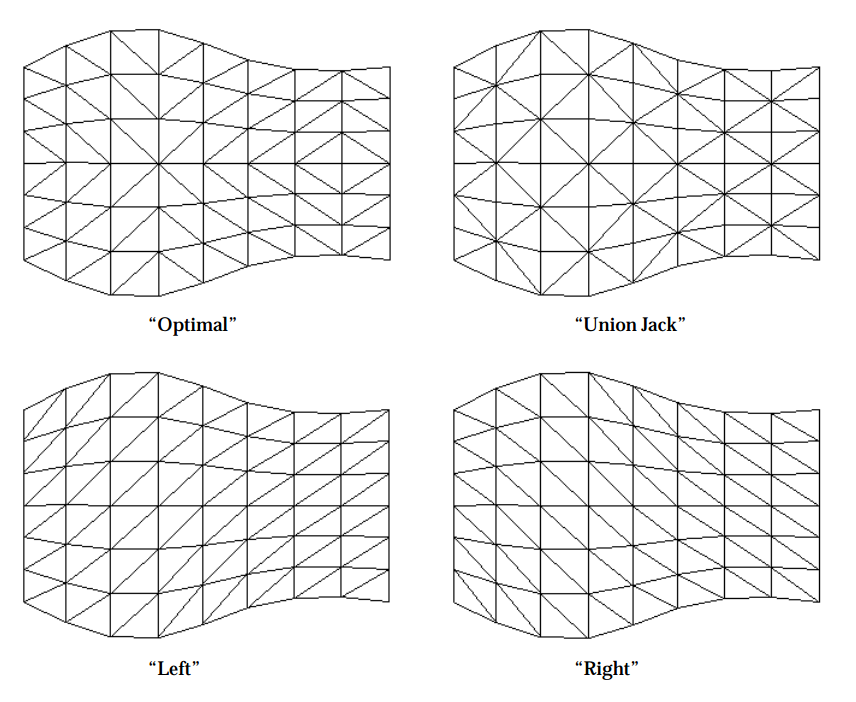
\includegraphics[scale = 0.6]{differentMeshes.png}}}
\centerline{Figure 1. Known Union-Jack Mesh Configuration}

\vspace{2mm}

\centerline {\frame{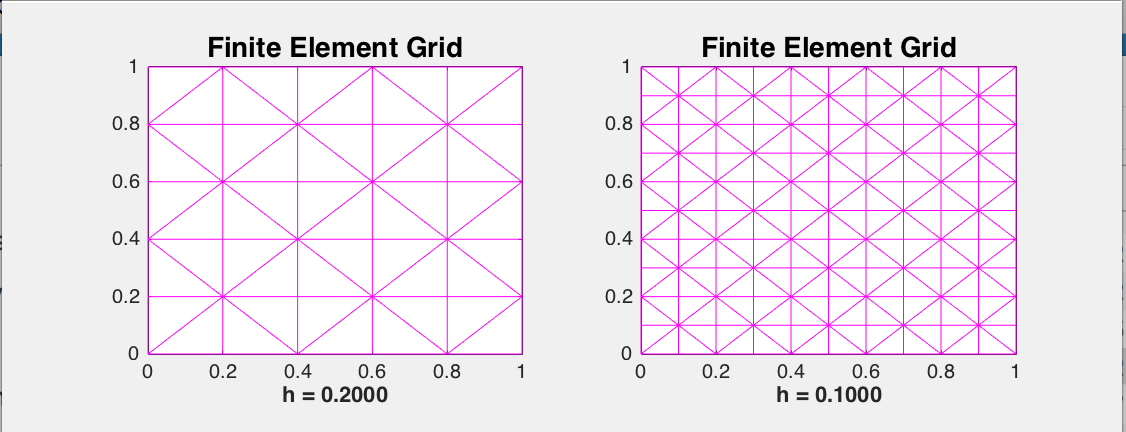
\includegraphics[scale = 0.6]{meshCompare.png}}}
\centerline{Figure 2. Comparison of Self-Made Union-Jack Mesh Configuration}

\vspace{5mm}

Now that there is a working mesh, I wanted to test if my solution was correct. To test this, I compared the exact solution of $u(x,y) = \sin(2\pi x)\sin(2\pi y)$ using $x$ and $y$ values made from the function \texttt{meshgrid} to my solutions when I computed the right hand side exactly and using the triangle centroid using the function \texttt{triplot} as seen in Figure 3. For the second system, from the defined boundary conditions I knew that the left hand side of the grid would be zero and the right hand side would be one with a gradient in between them. Originally, I had a yellow orb in the middle and knew that was incorrect. After fixing the boundary conditions, I knew I had the correct answer as seen in Figure 4.

\vspace{2mm}

\centerline {\frame{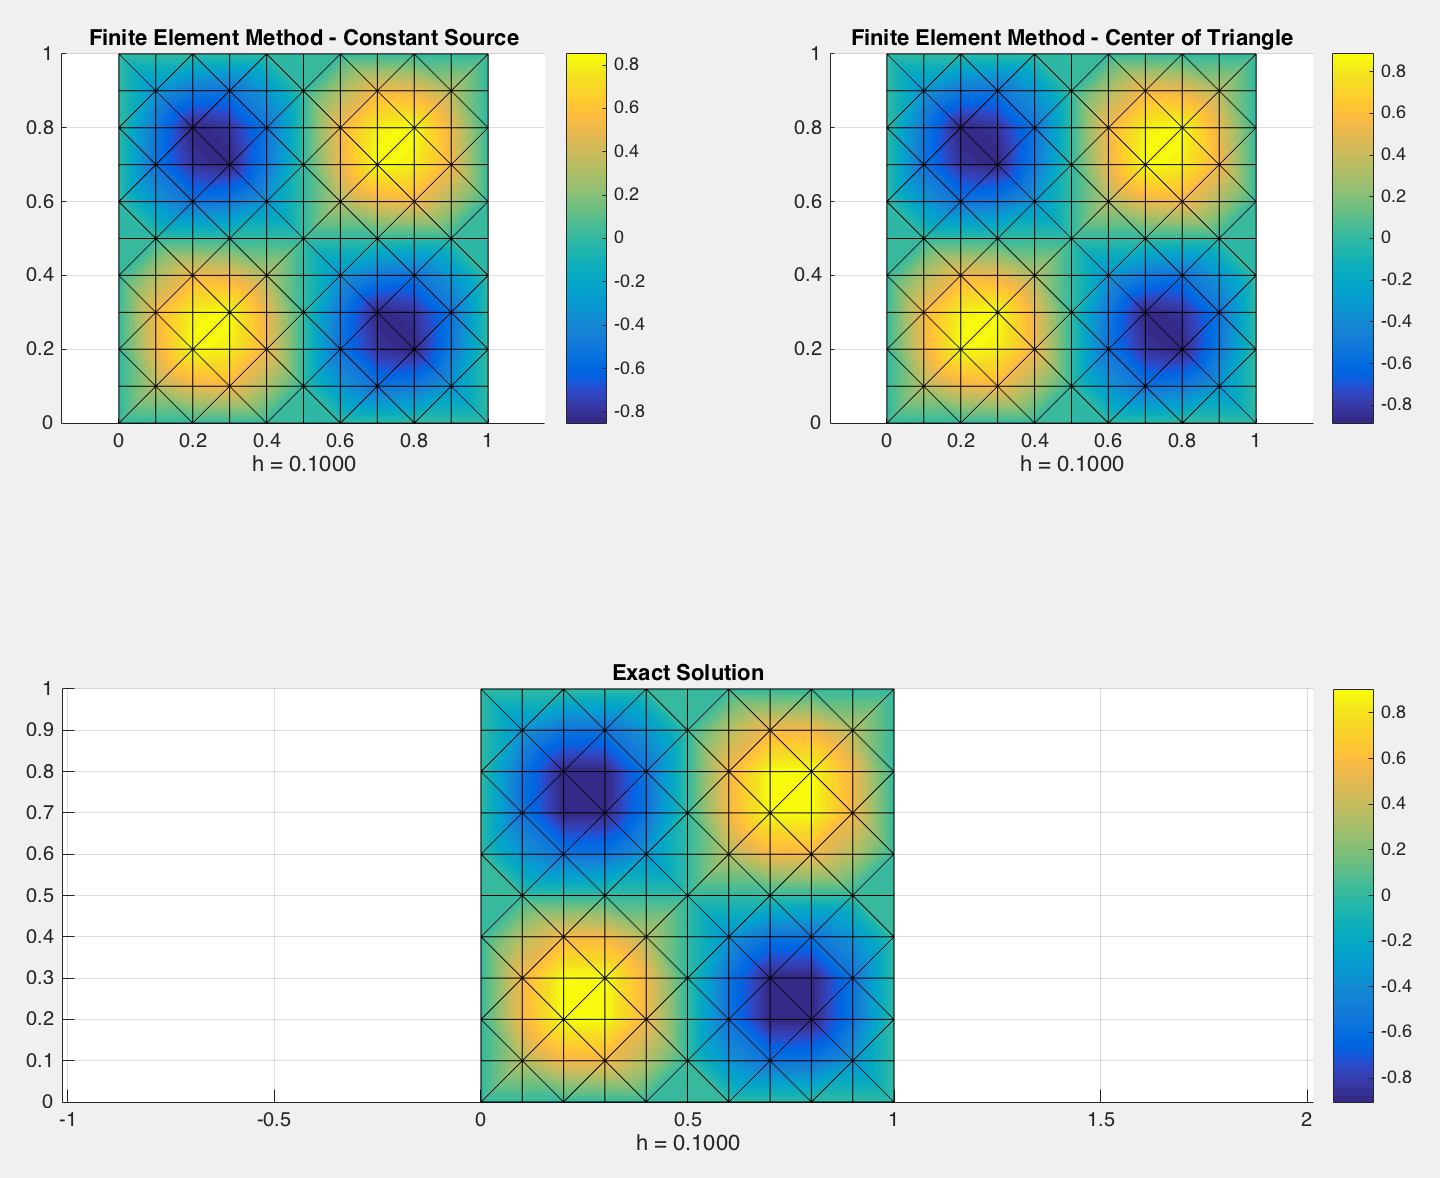
\includegraphics[scale = 0.7]{SolutionCompare.png}}}
\centerline{Figure 3. Comparison of Solutions}

\vspace{2mm}

\centerline {\frame{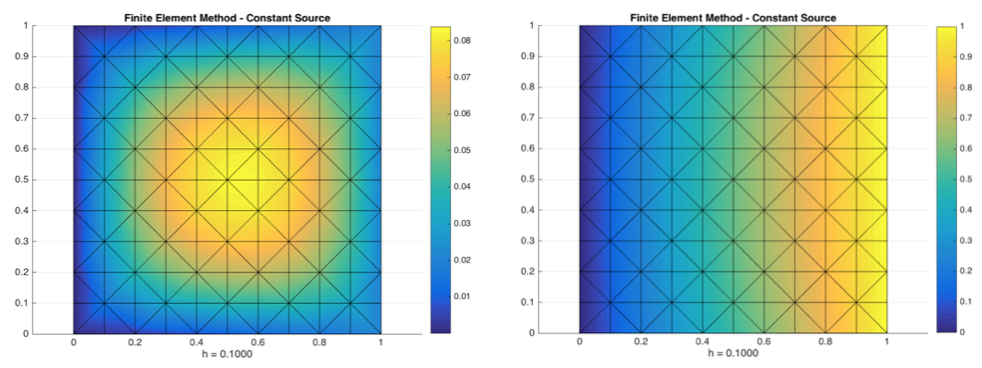
\includegraphics[scale = 0.5]{SolutionCompare_secondSystem.png}}}
\centerline{Figure 4. Comparison of Solutions - Second System}

\section{Results/Analysis of Results}

\subsection{Part 1}

The figures below show the solution of the first system solved with a 2D FEM solver at spacings $\frac{1}{5}$, $\frac{1}{10}$, $\frac{1}{20}$, $\frac{1}{40}$ and $\frac{1}{80}$ with the right hand side computed exactly and using element centroids compared to the true solution. 

The results are what was expected because it is on the same scale and looks like the exact solution. The results are consistent across finer mesh grids. As the mesh gets finer, the solution becomes more refined as well. 

Figure 10 shows the comparison of the error for the function evaluation and the triangle centroid, plotted with the spacing squared. The shape of the error is what we would expect; as the mesh gets finer, the error gets smaller.

\centerline {\frame{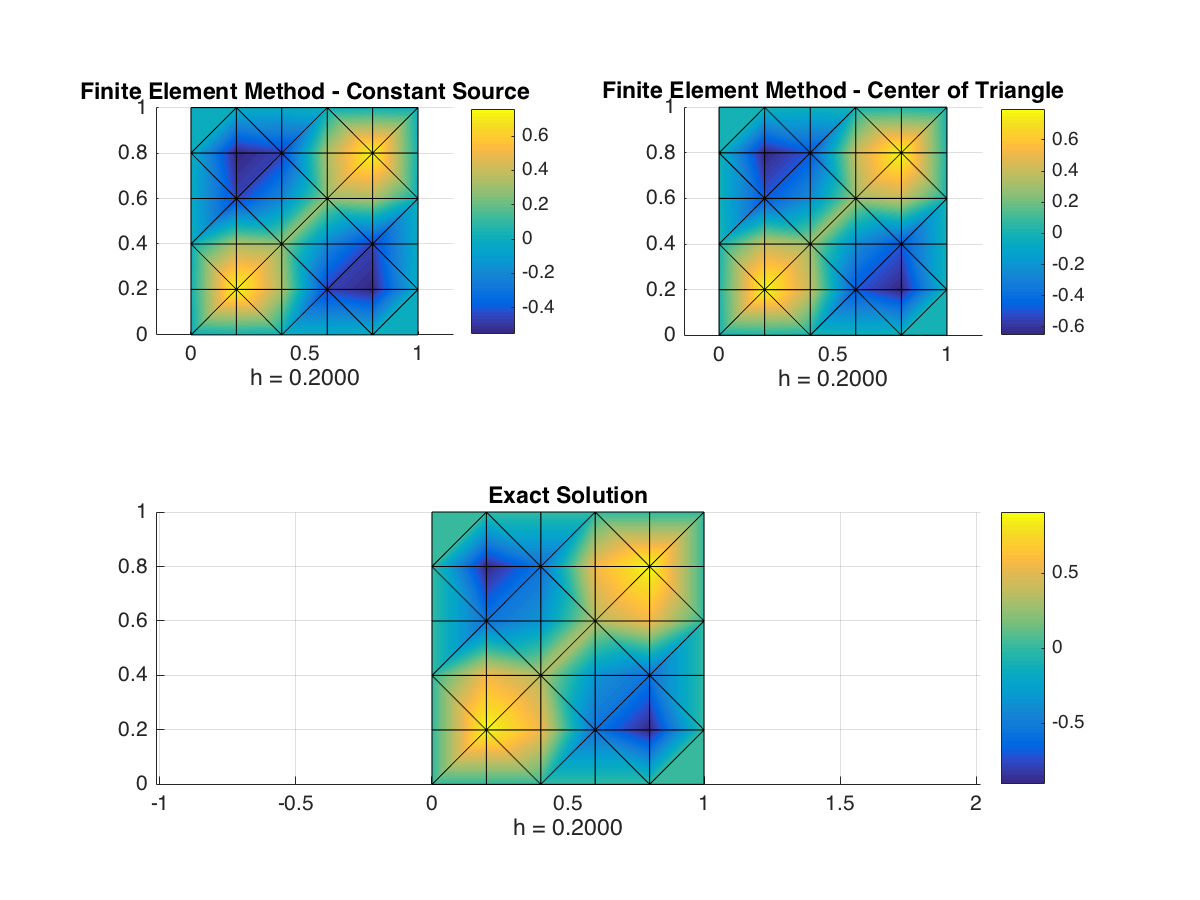
\includegraphics[scale = 0.6]{SolutionCompare_5.png}}}
\centerline{Figure 5. Comparison of Solutions - $h = \frac{1}{5}$}

\centerline {\frame{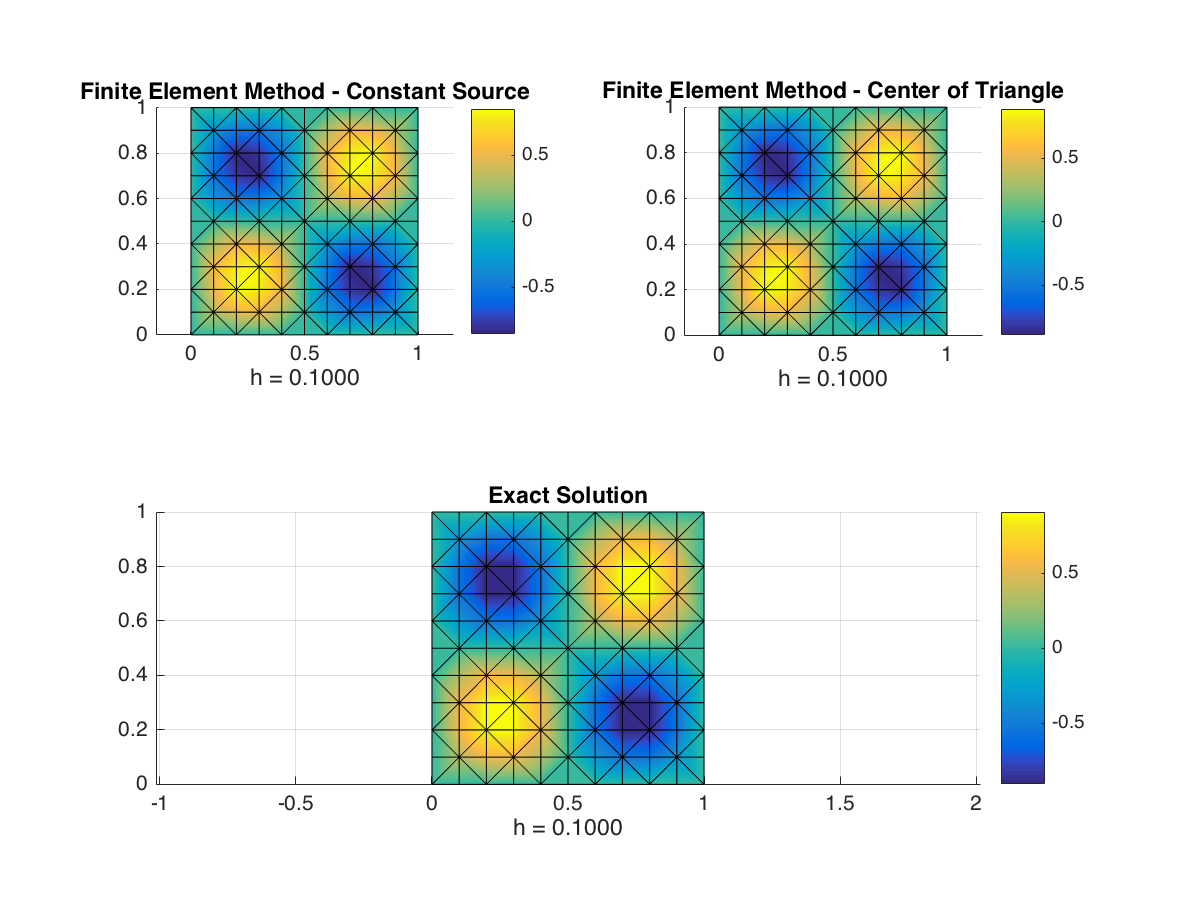
\includegraphics[scale = 0.6]{SolutionCompare_10.png}}}
\centerline{Figure 6. Comparison of Solutions - $h = \frac{1}{10}$}

\centerline {\frame{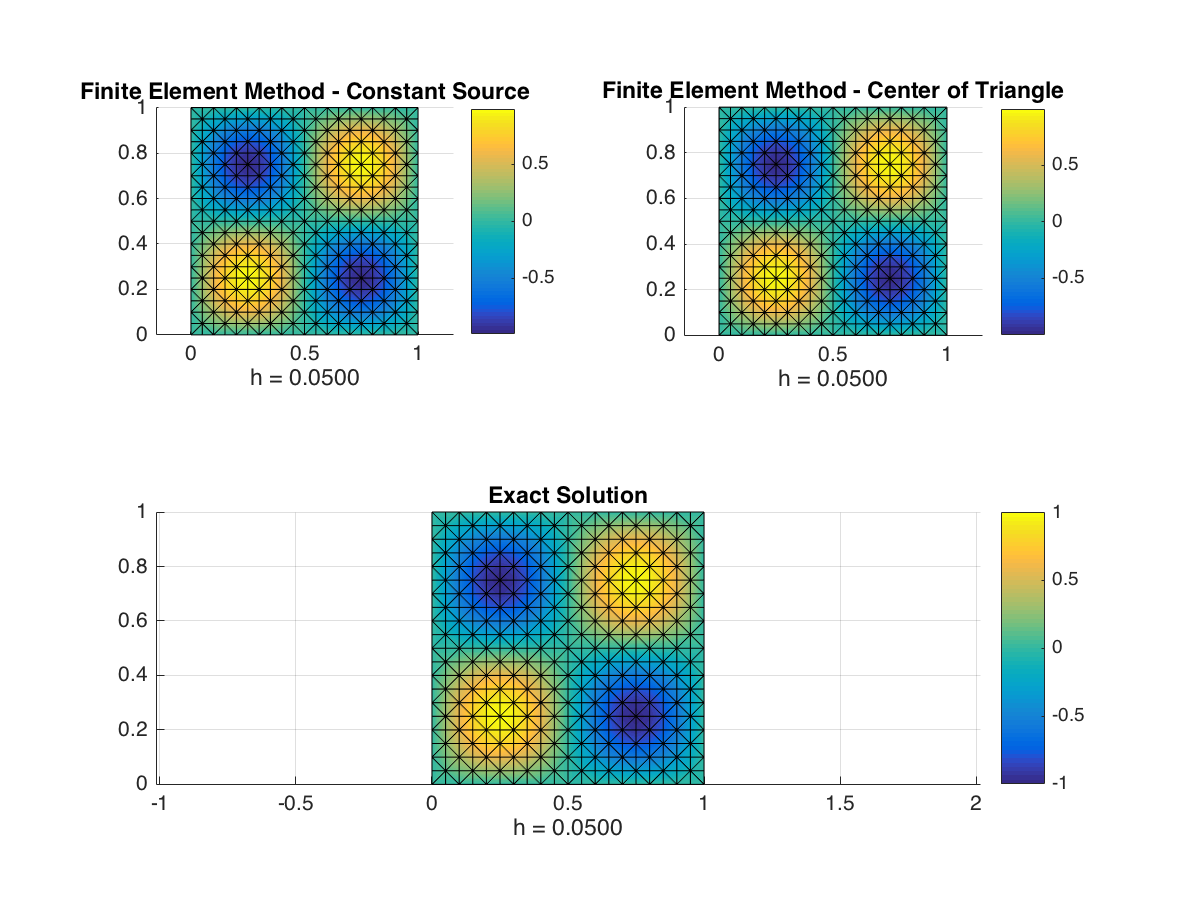
\includegraphics[scale = 0.6]{SolutionCompare_20.png}}}
\centerline{Figure 7. Comparison of Solutions - $h = \frac{1}{20}$}

\centerline {\frame{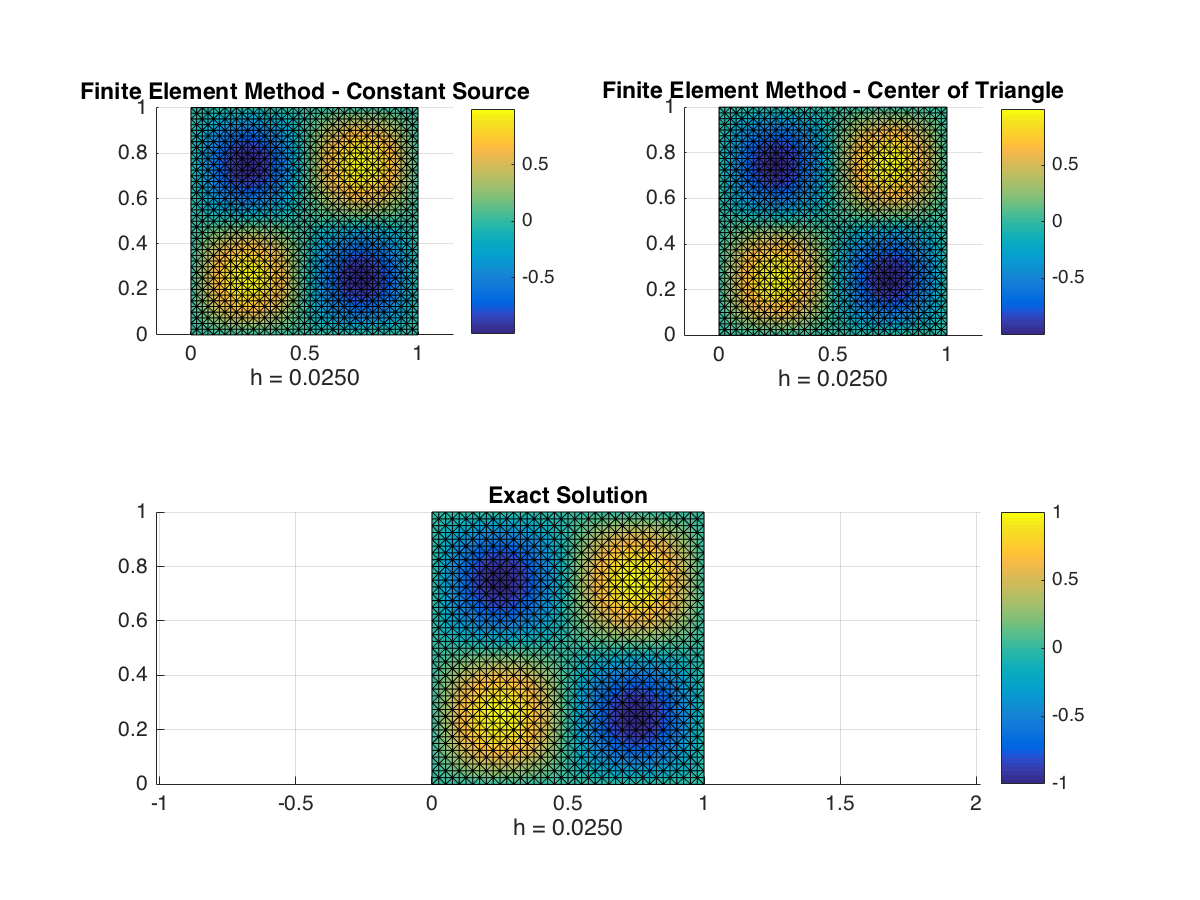
\includegraphics[scale = 0.6]{SolutionCompare_40.png}}}
\centerline{Figure 8. Comparison of Solutions - $h = \frac{1}{40}$}

\centerline {\frame{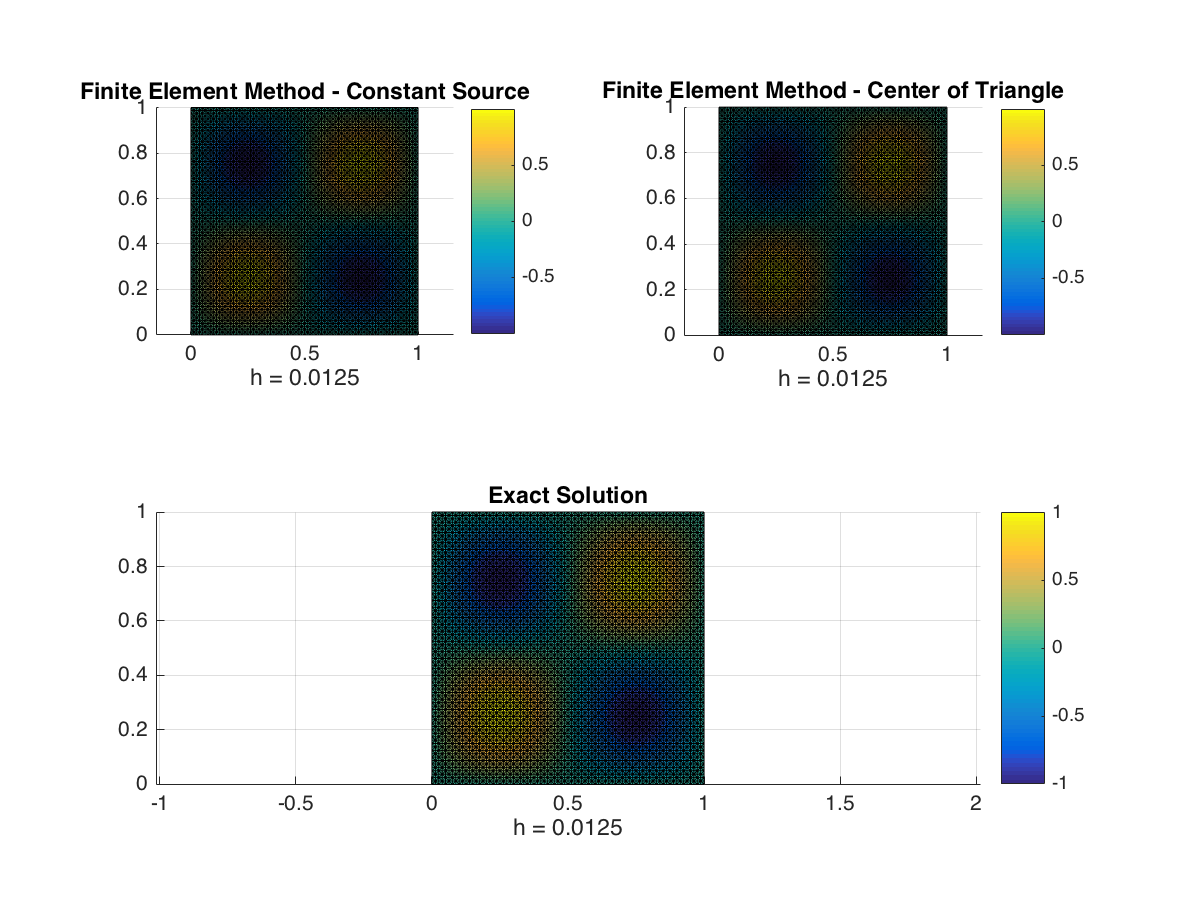
\includegraphics[scale = 0.6]{SolutionCompare_80.png}}}
\centerline{Figure 9. Comparison of Solutions - $h = \frac{1}{80}$}

\centerline {\frame{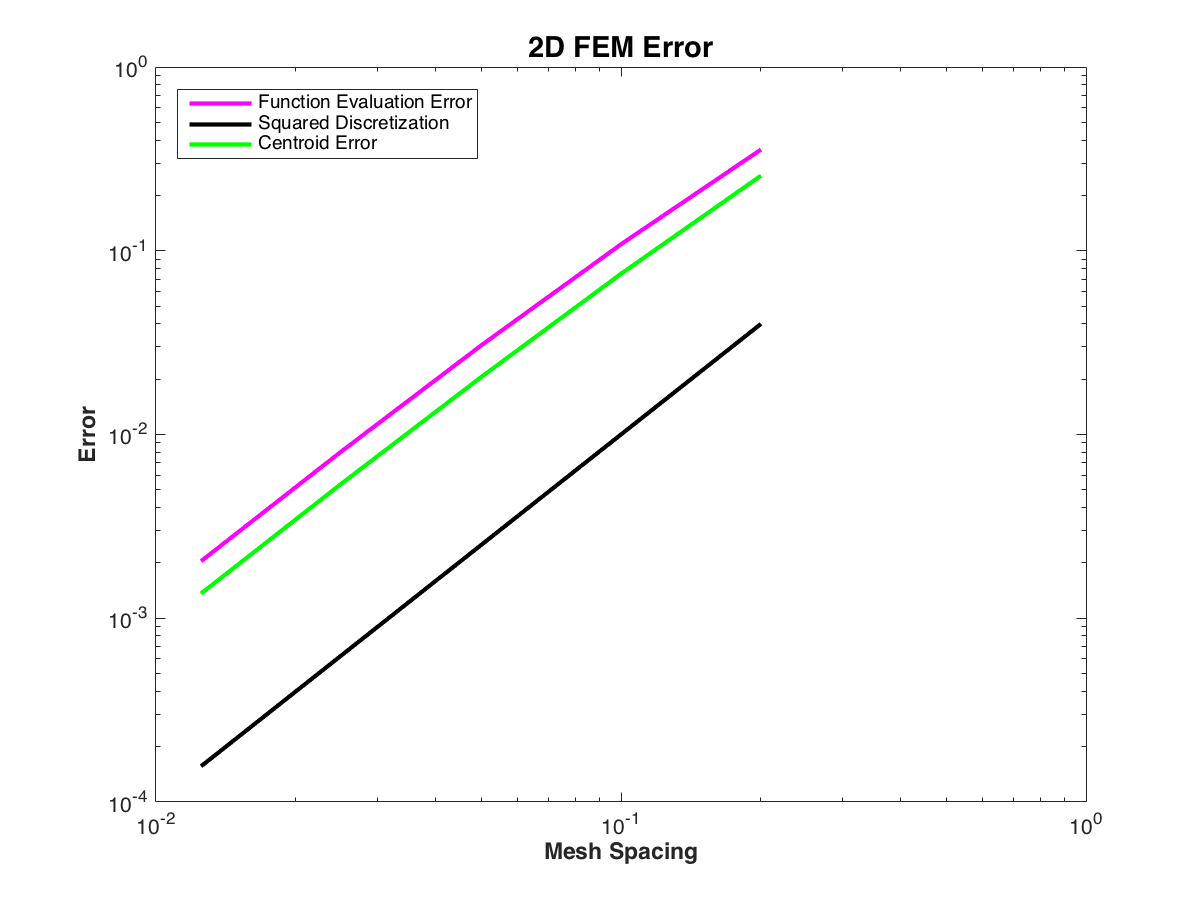
\includegraphics[scale = 0.6]{nonuniform_error_FEM.png}}}
\centerline{Figure 10. Comparison of Solutions - Max Error}

\subsection{Part 2}

The figures below show the results for the second system. These are the results I expected to see from this system, and the answer becomes finer with finer mesh spacings which is what I would expect as well.

\vspace{2mm}

\centerline {\frame{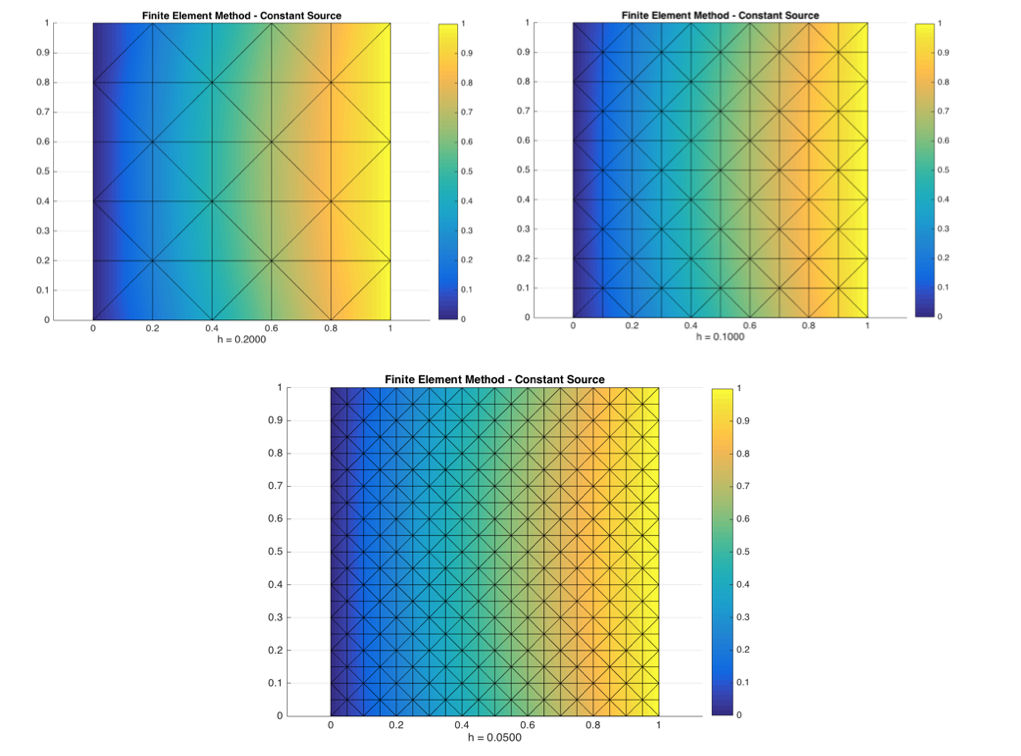
\includegraphics[scale = 0.4]{second_system_1.png}}}
\centerline {\frame{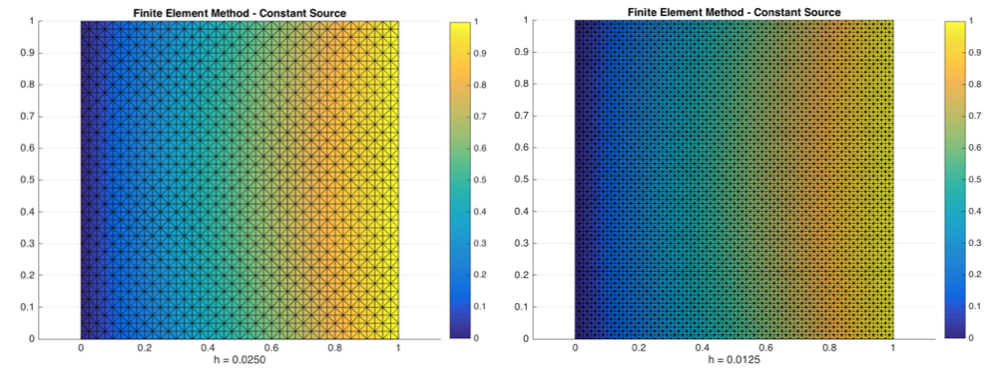
\includegraphics[scale = 0.42]{second_system_2.png}}}
\centerline{Figure 11. Comparison of Solutions at Different Mesh Spacings - Second System}

\section{Summary and Conclusions}

From Figure 10, we can see that 2D FEM is still second order accurate. The function evaluation, surprisingly, had slightly more error than the triangle centroid. As the mesh was refined, the solution also had less error and became more refined, as we can see from the figures. This can be easily seen with the second system due to the boundary conditions being equal to $x$, it gives a nice gradient that becomes much more refined as the mesh spacing becomes smaller.

For simple problems, FEM solvers have a lot of moving parts! Although I can see how this would break down a large and complex mesh into smaller problems because we look at it element by element.

\section{References}

\begin{enumerate}

\item Chris Johnson's CS 6220 class notes

\item The Finite Element Method using MATLAB, Young W. Kwon \& Hyochoon Bang

\end{enumerate}

\end{document}